
\part*{Potenzen}


\section*{Gesetze}

\begin{tabular}{|c|c|c|c|c|}
\hline 
$a^{n}\cdot a^{m}=a^{n+m}$ & $a^{n}:a^{m}=a^{n-m}$ & $a^{n}\cdot b^{n}=(a\cdot b)^{n}$ & $\frac{a^{n}}{b^{n}}=(\frac{a}{b})^{n}$ & $(a^{n})^{m}=a^{n\cdot m}$\tabularnewline
\hline 
$a^{-n}=\frac{1}{a^{n}}$ & $\sqrt[n]{a}=a^{\frac{1}{n}}$ & $\sqrt[n]{a^{m}}=(\sqrt[n]{a})^{m}=a^{\frac{m}{n}}$ & $-a^{n}=-(a^{n})$ & $(-a)^{n}=(-1)^{n}\cdot a^{n}$\tabularnewline
\hline 
\end{tabular}


\part*{Additionstheoreme}


\section*{Sätze}
\begin{itemize}
\item $sin(\alpha+\beta)=sin(\alpha)\cdot cos(\beta)+cos(\alpha)\cdot sin(\beta)$
\item $sin(\alpha-\beta)=sin(\alpha)\cdot cos(\beta)-cos(\alpha)\cdot sin(\beta)$
\item $cos(\alpha+\beta)=cos(\alpha)\cdot cos(\beta)+sin(\alpha)\cdot sin(\beta)$
\item $sin(\alpha-\beta)=cos(\alpha)\cdot cos(\beta)-sin(\alpha)\cdot sin(\beta)$
\end{itemize}

\part*{Trigonometrische Funktionen}


\section*{Definition}
\begin{verse}
\begin{tabular}{ll}
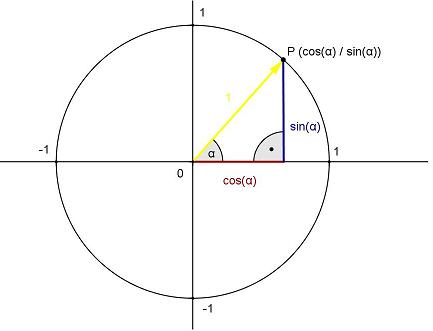
\includegraphics[height=6cm]{Repetition/Einheitskreis} & 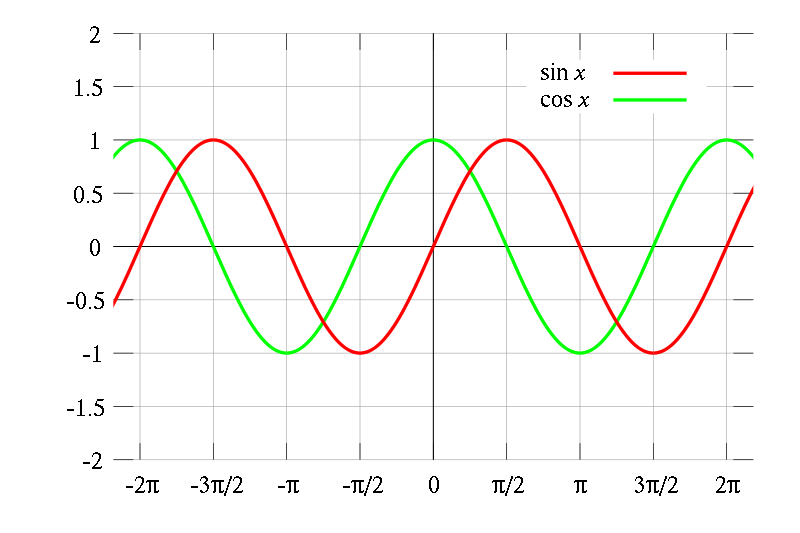
\includegraphics[height=6cm]{Repetition/Sin_Cos}\tabularnewline
\end{tabular}
\end{verse}
\begin{tabular}{|c|c|c|}
\hline 
$sin(x)=cos(x)\cdot tan(x)$ & $cos(x)=\frac{sin(x)}{tan(x)}$ & $tan(x)=\frac{sin(x)}{cos(x)}$\tabularnewline
\hline 
\end{tabular}


\section*{Bogenmass eines Winkels}

Länge des zugehörigen Bogens im Einheitskreis.
\begin{verse}
$\alpha=90\text{°}\leftrightarrow\alpha=\frac{\Pi}{2}$

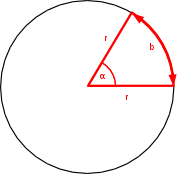
\includegraphics[height=3cm]{Repetition/Bogenmass}
\end{verse}

\section*{Anwendung in der Schwingungslehre}
\begin{verse}
\begin{tabular}{lll}
A = Amplitude & w = Kreisfrequenz & $\varphi$ = Phase der Schwingung\tabularnewline
 &  & Periode p = $\frac{alte\, Periode}{w}$, also bei sin/cos z.B.: $\frac{2\Pi}{w}$\tabularnewline
\end{tabular}

\begin{tabular}{|c|}
\hline 
$y=A\cdot sin[w\cdot t+\varphi]=A\cdot sin[\, w\cdot(t+\frac{\varphi}{w})\,]$\tabularnewline
\hline 
\end{tabular}
\end{verse}
Allgemein:
\begin{enumerate}
\item Streckung in y-Richtung mit Faktor a $\Rightarrow$ Wertebereich {[}-a,a{]}
\item Streckung in x-Richtung mit Faktor $\frac{1}{b}\Rightarrow$neue Periode
$\frac{alte\, Periode}{b}$, also bei sin/cos z.B.: $\frac{2\Pi}{b}$
\item Verschiebung in x-Richtung um $-\frac{\varphi}{b}$\end{enumerate}
\begin{verse}
\begin{tabular}{|c|}
\hline 
$y=a\cdot f[\, b\cdot(x-c)\,]+d$\tabularnewline
\hline 
\end{tabular}
\end{verse}
Beispiel:
\begin{verse}
\begin{tabular}{|c|}
\hline 
$y=3\cdot sin[\frac{1}{2}\cdot x+\frac{\Pi}{4}]=3\cdot sin[\,\frac{1}{2}\cdot(x+\frac{\Pi}{2})\,]$\tabularnewline
\hline 
\end{tabular}

\begin{tabular}{cccc}
Amplitude = 3 & Kreisfrequenz = $\frac{1}{2}$ & $\Rightarrow$Neue Periode = $\frac{2\Pi}{w}=\frac{2\Pi}{\frac{1}{2}}=4\Pi$ & Verschiebung in x-Richtung = $-\frac{\Pi}{2}$\tabularnewline
\end{tabular}

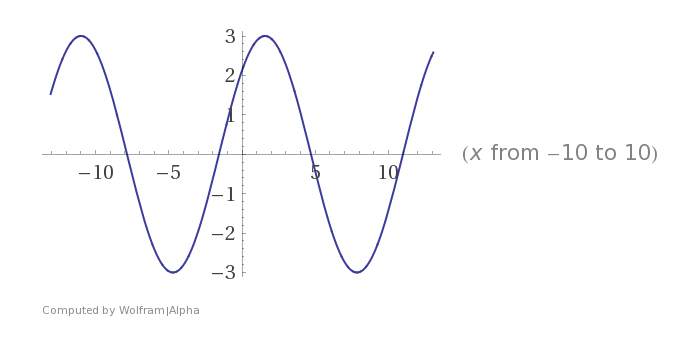
\includegraphics[height=5cm]{Repetition/Schwingung}
\end{verse}

\part*{Exponetial- und Logarithmusfunktion}

Jede Exponentielle Funktion lässt sich mit der Basis e schreiben:

\begin{tabular}{|c|}
\hline 
$y=b^{x}=(e^{ln(b)})^{x}$\tabularnewline
\hline 
\end{tabular}


\section*{Wachstums- und Zerfallfunktion}

Allgemein:

\begin{tabular}{ll}
$a=$Wert für $t^{0}$, ``Startwert'' & $b=$Wachstumsfaktor pro Zeiteinheit\tabularnewline
$t=$Zeiteinheit & $\Delta t=$Zeitdifferenz z.B. $t^{2}-t^{1}$\tabularnewline
\end{tabular}
\begin{verse}
\begin{tabular}{|c|}
\hline 
$y=a\cdot b^{t}$\tabularnewline
\hline 
\end{tabular}

\begin{tabular}{cc}
\textbf{Wachstumsfunktion: b > 1,} & \textbf{Zerfallsfunktion: 0 < b < 1 }\tabularnewline
\end{tabular}
\end{verse}
Umformungen:
\begin{verse}
\begin{tabular}{|c|}
\hline 
$b^{\Delta t}=\frac{f(t_{2})}{f(t_{1})}\Rightarrow b=\sqrt[\Delta t]{\frac{f(t_{2})}{f(t_{1})}}$\tabularnewline
\hline 
\end{tabular}
\end{verse}
Halbwertszeit:
\begin{verse}
\begin{tabular}{|c|}
\hline 
$b^{\Delta t}=\frac{1}{2}\Rightarrow\Delta t\cdot ln(b)=ln(\frac{1}{2})\Rightarrow\Delta t=\frac{ln(\frac{1}{2})}{ln(b)}$\tabularnewline
\hline 
\end{tabular}
\end{verse}
Verdoppelungszeit:
\begin{verse}
\begin{tabular}{|c|}
\hline 
$b^{\Delta t}=2\Rightarrow\Delta t\cdot ln(b)=ln(2)\Rightarrow\Delta t=\frac{ln(2)}{ln(b)}$\tabularnewline
\hline 
\end{tabular}
\end{verse}

\section*{Logarithmusfunktion}

Rechenregeln:
\begin{verse}
\begin{tabular}{|c|}
\hline 
$log_{a}(u\cdot v)=log_{a}(u)+log_{a}(v)$\tabularnewline
\hline 
$log_{a}(\frac{u}{v})=log_{a}(u)-log_{a}(v)$\tabularnewline
\hline 
$log_{a}(u^{k})=k\cdot log_{a}(u)$\tabularnewline
\hline 
$log_{a}(\sqrt[n]{u})=\frac{1}{n}\cdot log_{a}(u)$\tabularnewline
\hline 
\end{tabular}
\end{verse}
Allgemein:
\begin{verse}
\begin{tabular}{|c|}
\hline 
$y=a^{x}\Rightarrow ln(y)=x\cdot ln(a)\Rightarrow x=\frac{ln(y)}{ln(a)}$\tabularnewline
\hline 
\end{tabular}

\begin{tabular}{|c|}
\hline 
$y=a^{x}\Rightarrow log_{a}(y)=x\cdot log_{a}(a)\Rightarrow x=log_{a}(y)$ \tabularnewline
\hline 
\end{tabular}
\end{verse}
Umkehrfunktion:
\begin{verse}
\begin{tabular}{|c|}
\hline 
$y=log_{a}(x)$\tabularnewline
\hline 
\end{tabular}
\end{verse}
Basiswechsel:
\begin{verse}
\begin{tabular}{|c|}
\hline 
$log_{a}(x)=\frac{log_{10}(x)}{log_{10}(a)}=\frac{ln(x)}{ln(a)}$\tabularnewline
\hline 
\end{tabular}
\end{verse}
Umformungsbeispiele:
\begin{verse}
\begin{tabular}{|l|l|l|}
\hline 
$log_{10}(x)=-4.0404$ & $\Rightarrow$ & $x=10^{-4.0404}=\frac{1}{10^{4.0404}}$\tabularnewline
\hline 
$ln(x)=-9.0907$ & $\Rightarrow$ & $x=e^{-9.0907}=\frac{1}{e^{9.0907}}$\tabularnewline
\hline 
$log_{3}(x)=5$ & $\Rightarrow$ & $x=3^{5}=243$\tabularnewline
\hline 
\end{tabular}\end{verse}

